\section{Proposed occupancy estimation approaches}
\label{sec:proposed_methods}
In this section we apply the SVR and RNN methods on occupancy estimation in a smart building that contains 5 zones. The whole smart building is simulated by using the energy simulation tool EnergyPlus. We will first discuss the principles based on the features used for detection and then conduct the data configuration used in the model for occupancy detection.
\subsection{Feature Selection}
\begin{figure}[h]
\centering
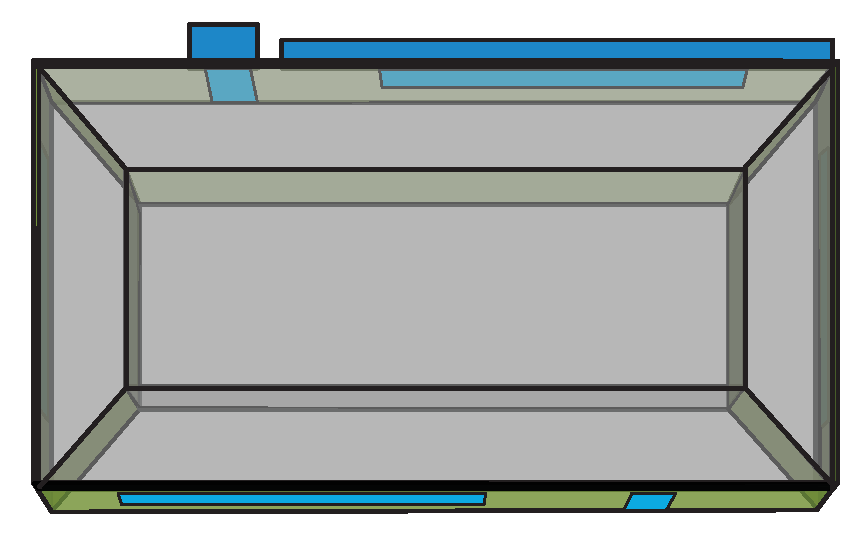
\includegraphics[width=4in]{./Pics/TopView2.eps}
\caption{The office model: top view.}
\label{fig:office1}
\end{figure}

\begin{figure}[h]
\centering
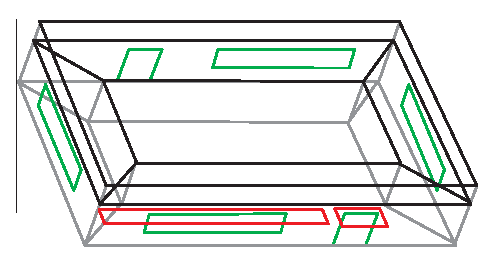
\includegraphics[width=4in]{./Pics/SideView.eps}
\caption{The office model: side view.}
\label{fig:office2}
\end{figure}

\begin{figure}[h]
\centering
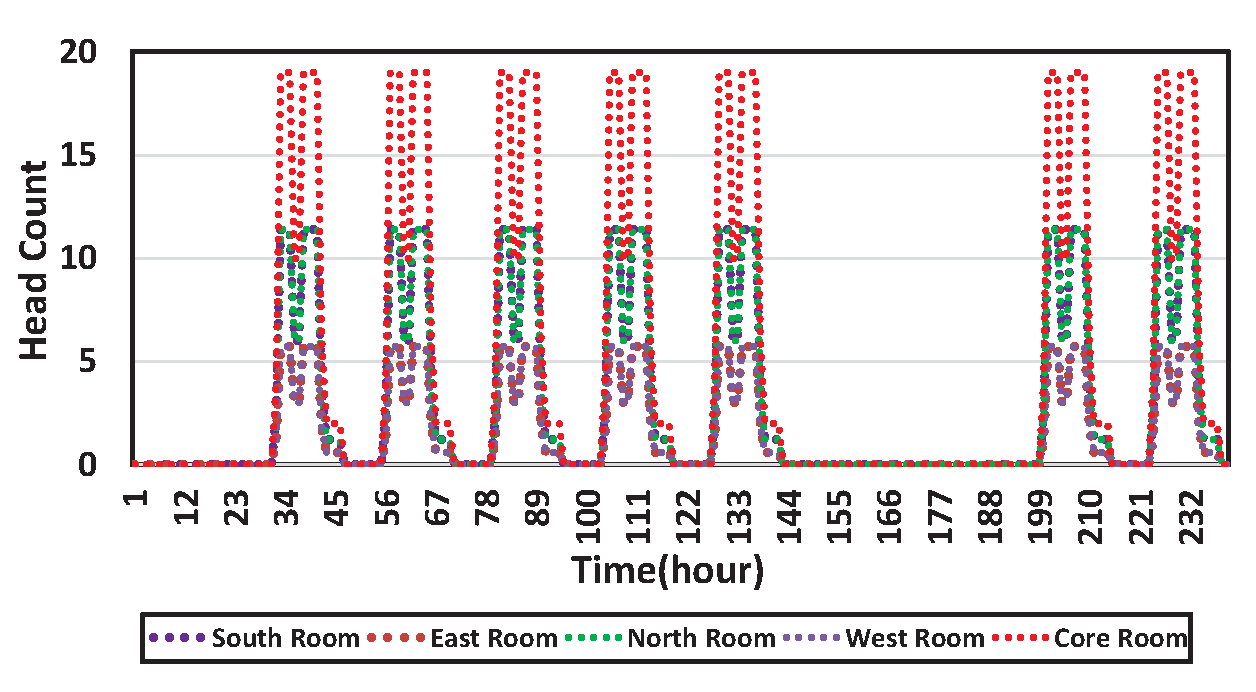
\includegraphics[width=4in]{./Pics/Headcount.eps}
\caption{Occupation information of 5 rooms for 10 days.}
\label{fig:Headcount}
\end{figure}

\begin{figure}[h]
\centering
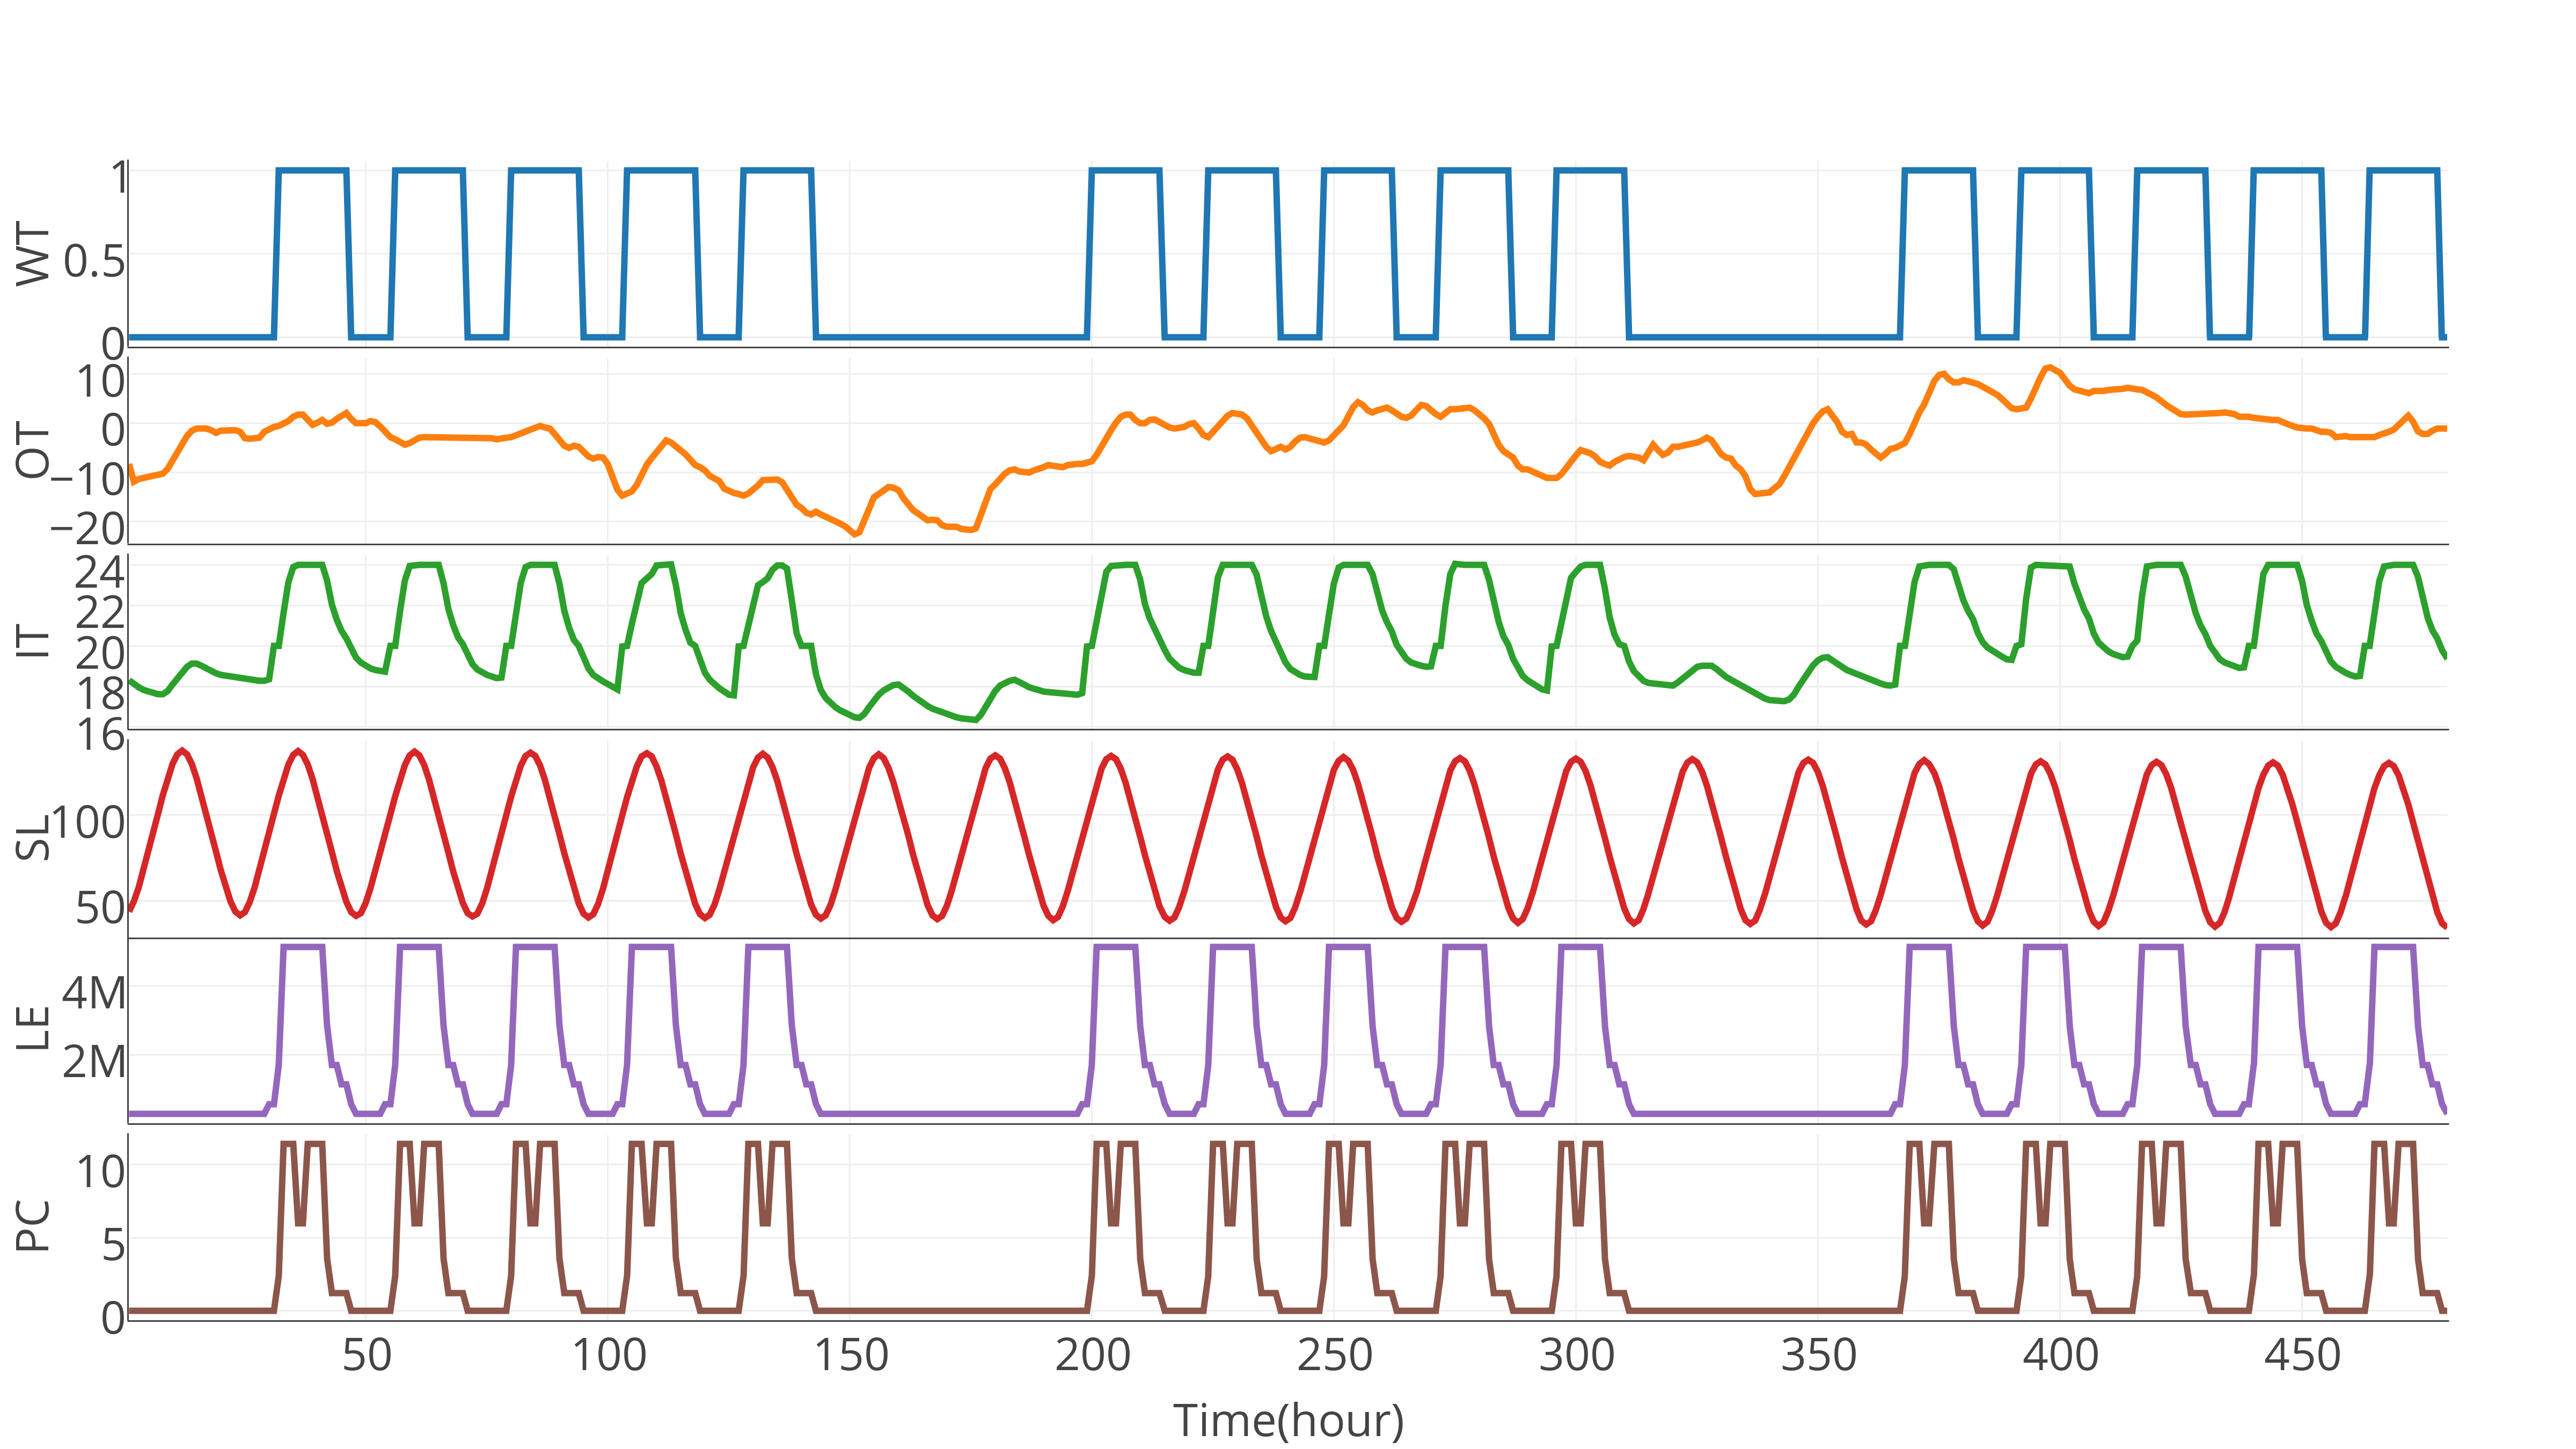
\includegraphics[width=4in]{./Pics/Feature3.eps}
\caption{Selected EnergyPlus input and simulated temperature output data sample in 20 days. (WT: Work time; OT: Outdoor temperature; IT: Indoor temperature; SL: Solar angle; LE: Lights energy; PC: People count.)}
\label{fig:feature}
\end{figure}

In the machine learning model we built for occupancy detection, we
carefully selected 5 features each of which possesses some unique
information hidden inside. The features are solar angle, indoor
temperatures, outdoor temperatures, working time, and lights energy.
Solar angle is believed to have periodic information which varies
across the entire year, outdoor temperature is an apparent factor that
impacts the indoor temperature, working time denotes whether regular
working schedule is executed, and lights energy gives out a radiation
metric that causes rise of the temperature.

Fig.~\ref{fig:office1} and Fig.~\ref{fig:office2} show the side view
and the top view of the building which contains five rooms and HVAC
system by using the software EnergyPlus. This building can be
influenced by heat sources produced from occupants, electric
equipment, air filtration, etc. The weather (ambient temperature and
solar effects) affects the room temperature as well. Through the HVAC
system with coil and fan, room temperature can be administered
properly to ensure that a comfortable temperature in the environment
can be produced in the room.

In this room the solar angle ${\theta _s}$ is defined as the angle between the zenith and the centre of the sun disc
\begin{equation}
    \cos {\theta _s} = \sin \phi \sin \delta  + \cos \phi \cos \delta \cosh
\end{equation}
where $h$ is the hour angle in the local solar time, $\delta$ is the
current declination of the sum, and $\phi$ is the local latitude. This
equation enables us to compute the feature solar angle and all the
variables are correlated to the location of the building.

Working time is a feature that determines if the time detected is
local working time or not, and it apparently affect the number of
working people in a certain office. It is also convenient to achieve
schedule of an ordinary worker in an office within the building and it
is a good feature contributing to the detection. When a feature is
being considered to be incorporated in the feature pool, we first
figure out the convenience and difficulty in acquiring the data set.
Here the working time has a strong correlation with the employee common
schedule, which is a relatively data set to acquire. Therefore, the
working time is chosen as a feature element in the feature pool, and
it is even a basic feature owing to its convenience.

Outdoor temperatures are off-the-rack data set collected from weather
forecast which also are the inputs for EnergyPlus to generate indoor
temperatures data as an output. Herein we use the outdoor
temperature data set of the location of the building simulated by EnergyPlus, so as
our simulated building model goes through the exact same weather
conditioning the genuine building has gone through. Outdoor
temperatures also plays an instrumental feature role in detection,
because it directly influences the indoor temperature, which has a
non-linear relationship with the number of employees in a certain
office.

The indoor temperature turns out to be one of the key features used in
the detection model, to be more accurately, all of the factors
including employee occupancy constitute the list of elements that
results in the fluctuation of temperature inside the building. In
essence, the approach to achieve the detection for a number of
employee in a certain room is based on the contribution of heat
emitted from different number of employees in a certain room. Owing to
the fact that different number of employees gives out different amount
of heat to impact the indoor temperature makes the approach viable to
detect the occupancy combing other factors that affect the indoor
temperature.

Lights energy is the fifth feature in the feature pool, and it is
different from the first four features. The first four features are quite
convenient features to acquire where the measurement of lights energy
is comparatively inconvenient to acquire. However, we want to make the
detection more versatile and can be applied in different situations.
Despite the inconvenience of data set of lights energy, it is an
important metric related to the number of employees in a specific office
as well. Aiming at provide a more accurate detection, the lights
energy feature is incorporated into the feature pool.

\textcolor{feb18rev}{As listed above, five main features are applied in the machine learning methods for occupancy detection. 
These features covers all major thermal-related aspects to be coupled with the human activity, such that
occupancy can be determined theoretically. In order to investigate the impact
of choosing different set of features and to improve the flexibility of practical
deployment, different combination of features are used in the methods.}

\subsection{Data Configuration}
\begin{figure}[!h]
\centering
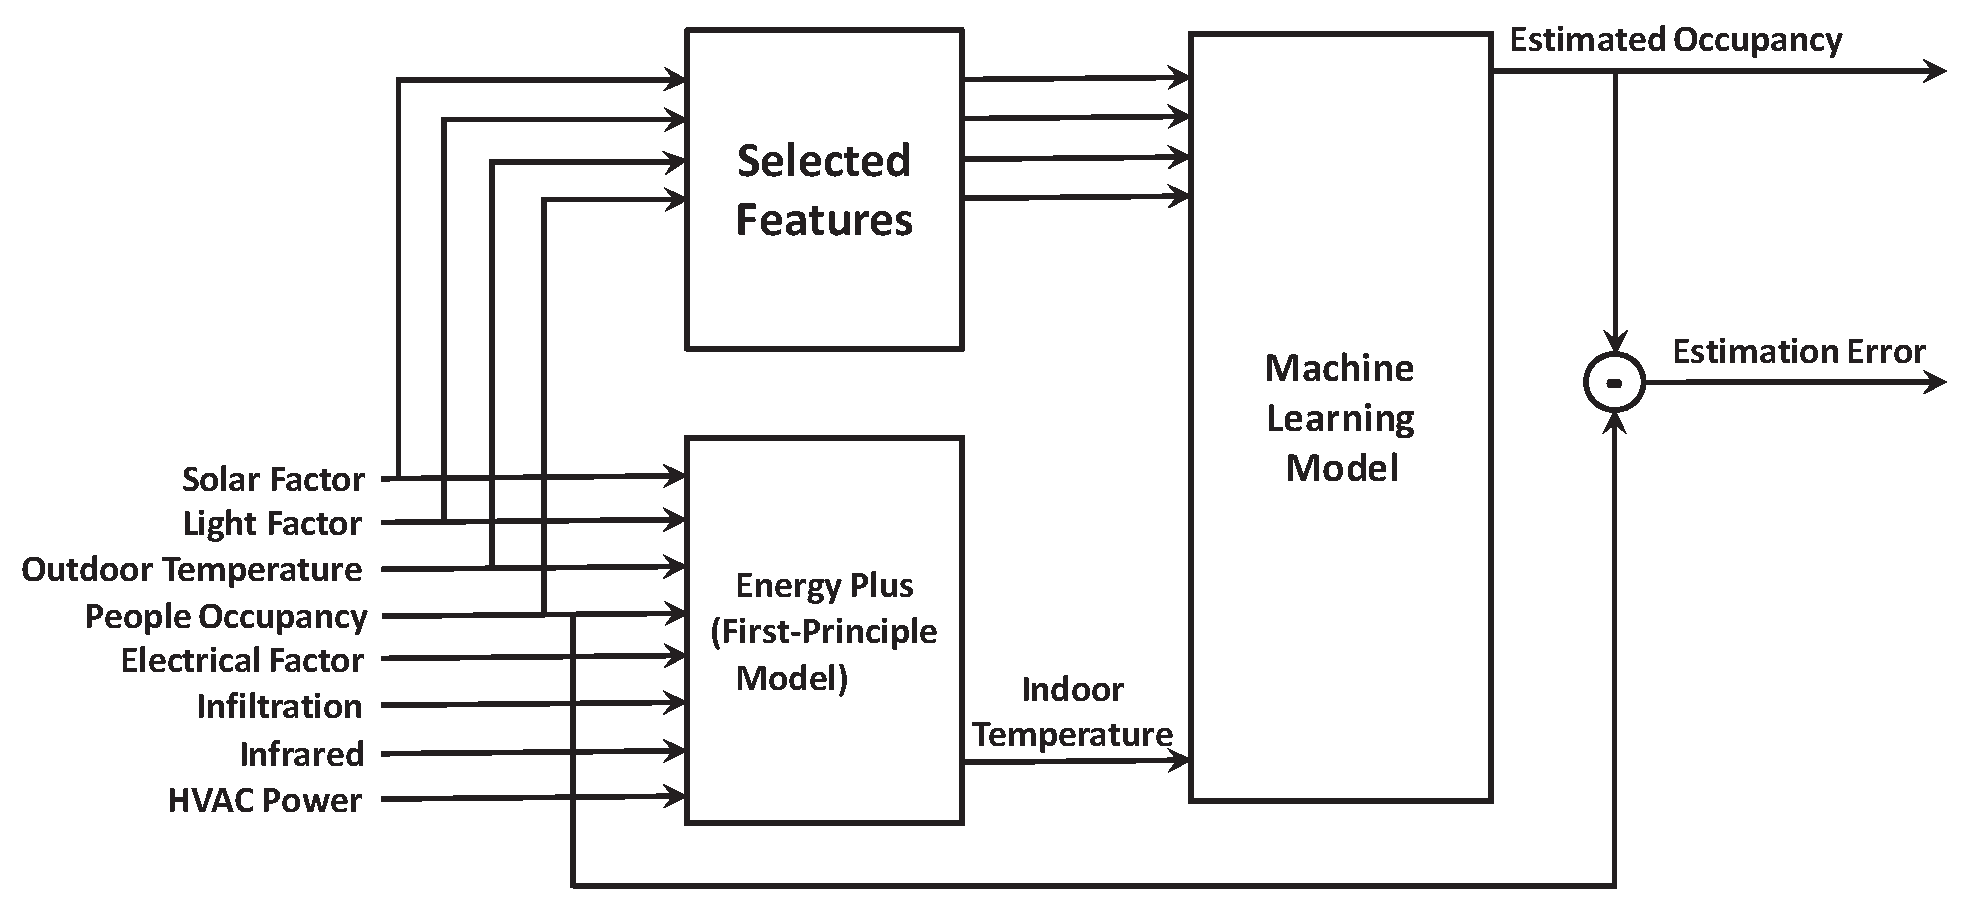
\includegraphics[width=4in]{./Pics/FlowDiagram2.eps}
\caption{Data configuration of machine learning model.}
\label{fig:SVRFlow}
\end{figure}

Fig.\ref{fig:SVRFlow} shows how EnergyPlus produces indoor temperature
in a certain room specifically. EnergyPlus feeds off factors such as
indoor temperature, solar factor, electrical factor, light factor,
infiltration, infrared, and people occupancy before it produces indoor
temperature as an output using built-in methods and methods in
accordance with its inputs. Of all those features taken into the
method, indoor temperature is the key feature because it is directly
impacted by the increase or drop in the number of employees in a
certain office.

In general, the machine learning model takes the selected parameters
as its features to train the data and yield results. It is highlighted
that the relationship between occupancy and other factors are
non-linear related, where SVR and RNN are good choices to
solve a non-linear problem used for detection. Machine learning methods are
increasingly used in all kinds of supervised and unsupervised problems
in all aspects.

Fig.~\ref{fig:Headcount} shows a vintage working schedule of the five
zones of an office building. Our goal of the detection model is to
detect accurate number of employees in a room by certain parameters
and data collections. Fig.~\ref{fig:feature} shows the simulated
temperature curves and input curves over 20 days from EnergyPlus for a
smart building model with the five separate zones shown in
Fig.~\ref{fig:office2}. The schedule for each room can be assigned
differently by EnergyPlus. The selected features are then combined
together to occupancy behavior in the smart building. In general, the
SVR model takes the selected features as its parameters to train the
data and yield the corresponding results. It should be noted that
there is a nonlinear relationship between the occupancy and the
related factors. The machine learning model can be used to solve this
nonlinear problem for occupancy detection.

%In this model, we provide two sets of model which offers different
%extent of convenience to detect number of employees in an office. The
%first set of model is comprised of features such as solar factor,
%working time, indoor temperature and outdoor temperature, data of
%which can be acquired through sole mathematic computation and
%EnergyPlus simulation. It is relatively convenient to obtain all the
%features required in the first feature set. However, we introduce one
%more features in the second feature set, light factor, to enhance the
%accuracy of model. Light factor requires the model to learn overall
%energy that light consumes during a certain quantity of time which is
%a comparatively inconvenient feature to obtain, however, it is capable
%of making the detection more accurate. It is also highlighted here
%that all of the data we feed in the model is generated from EnergyPlus
%or obtained through mathematical calculation, thus further experiments
%are likely to be conducted in real-life data condition.

\textcolor{feb18rev}{In the proposed machine learning model, two features sets are provided
for occupancy detection in a building. The first set is comprised of features such as solar factor,
working time, indoor temperature and outdoor temperature, which can be acquired through sole mathematic computation and
EnergyPlus simulation.} It is relatively convenient to obtain all the
features required in the first feature set. However, we introduce one
more feature in the second feature set, light factor, to enhance the
accuracy of model. Light factor requires the model to learn overall
energy that light consumes during a certain quantity of time which is
a comparatively inconvenient feature to obtain, however, it is capable
of making the detection more accurate. It is also highlighted here
that all of the data we feed in the model is generated from EnergyPlus
or obtained through mathematical calculation, thus further experiments
are likely to be conducted in real-life data condition.

For separating the whole data set, we split the one-year simulation
data into twelve months and three time periods, in which the months
1-3, 5-7, 9-11 are referred to as the training data and the months 4,
8, 12 are specified for the testing data in the proposed machine
learning model.
